% Created 2019-06-16 Sun 09:30
% Intended LaTeX compiler: pdflatex
\documentclass[presentation]{beamer}
\usepackage[utf8]{inputenc}
\usepackage[T1]{fontenc}
\usepackage{graphicx}
\usepackage{grffile}
\usepackage{longtable}
\usepackage{wrapfig}
\usepackage{rotating}
\usepackage[normalem]{ulem}
\usepackage{amsmath}
\usepackage{textcomp}
\usepackage{amssymb}
\usepackage{capt-of}
\usepackage{hyperref}
\usepackage{tabu}
\usepackage{minted}
\usepackage[english]{babel}
\hypersetup{pdfauthor="Vasilij Schneidermann", pdftitle="Knowing just enough crypto to be dangerous", colorlinks, linkcolor=, urlcolor=blue}
\setminted{fontsize=\footnotesize,escapeinside=@@}
\usetheme{Rochester}
\usecolortheme[RGB={87,83,170}]{structure}
\author{Vasilij Schneidermann}
\date{June 2019}
\title{Knowing just enough crypto to be dangerous}
\hypersetup{
 pdfauthor={Vasilij Schneidermann},
 pdftitle={Knowing just enough crypto to be dangerous},
 pdfkeywords={},
 pdfsubject={},
 pdfcreator={Emacs 26.2 (Org mode 9.1.9)}, 
 pdflang={English}}
\begin{document}

\maketitle
\begin{frame}{Outline}
\tableofcontents
\end{frame}

\AtBeginSection{\frame{\sectionpage}}

\section{Intro}
\label{sec:org566d422}

\begin{frame}[label={sec:org1d30ba4}]{About}
\begin{itemize}
\item Vasilij Schneidermann, 26
\item Software developer at bevuta IT, Cologne
\item mail@vasilij.de
\item \url{https://github.com/wasamasa}
\item \url{http://emacshorrors.com/}
\item \url{http://emacsninja.com/}
\end{itemize}
\end{frame}

\begin{frame}[label={sec:org583030f}]{Motivation}
\begin{itemize}
\item The current state of crypto is worrisome
\item More attacks found than ever
\item Rise in papers on side-channel attacks
\item Yet: Most people ignore crypto or focus on a specific application
(like, crypto currencies)
\item How does one learn it?
\item How hard can it be?
\end{itemize}
\end{frame}

\begin{frame}[label={sec:org36fe053}]{Context}
\begin{itemize}
\item Looking for programming challenges, most were boring
\item Cryptopals challenges:
\begin{itemize}
\item Well designed, incremental
\item Cover several fields (symmetric/asymmetric crypto, signing, PRNG,
hashing, zero-knowledge proofs, protocols/handshakes)
\item Programming language doesn't matter
\item Can be completed offline
\item You measure your own progress
\end{itemize}
\end{itemize}
\end{frame}

\begin{frame}[label={sec:org8b26012}]{Basics}
\begin{itemize}
\item Confidentiality, Integrity, Authenticity
\item Symmetric and asymmetric cryptography
\item Plaintext, ciphertext
\item Key, IV, nonce
\item Block and stream cipher modes
\end{itemize}
\end{frame}

\section{Selected attacks}
\label{sec:org3070d11}

\begin{frame}[label={sec:orgcf0276e}]{Candidates}
\begin{itemize}
\item Crack an MT19937 seed
\item Single-byte XOR cipher
\item CBC bitflipping attacks
\item Break “random access read/write” AES CTR
\item Compression Ratio Side-Channel Attacks
\end{itemize}
\end{frame}

\begin{frame}[label={sec:org31edd22}]{Picking a suitable programming language}
\begin{itemize}
\item I went for Ruby
\begin{itemize}
\item Expressive
\item Extensive standard library
\item Covers all prerequisites (OpenSSL, bignums)
\item Chance to improve my Ruby skills
\end{itemize}
\end{itemize}
\end{frame}

\begin{frame}[label={sec:org30dcf5b}]{Crack an MT19937 seed}
\begin{itemize}
\item This one doesn't even involve crypto
\item MT19937 is a very popular PRNG
\item Some people use it for crypto\ldots{}
\item Some people seed it from the current time\ldots{}
\item Given a MT19937 output seeded with a UNIX timestamp from a few
minutes ago, how do you figure out the seed?
\end{itemize}
\end{frame}

\begin{frame}[fragile,label={sec:orgbc5405b}]{Crack an MT19937 seed}
 \begin{minted}[]{ruby}
def random_number(seed)
  Random.new(seed).rand(2**32)
end

now = Time.now.to_i
seed = now - 123
rng_output = random_number(seed)
\end{minted}
\end{frame}

\begin{frame}[label={sec:org7990742}]{Crack an MT19937 seed}
\begin{itemize}
\item PRNG generates a specific sequence of numbers for a given seed
\item If you use the same seed as for a previous run, you get the same numbers
\item Idea: Try possible timestamps as seed values, check whether
first generated number matches up
\end{itemize}
\end{frame}

\begin{frame}[fragile,label={sec:orgf13ad9d}]{Crack an MT19937 seed}
 \begin{minted}[]{ruby}
def crack_it(start_time, rng_output)
  seed = start_time
  loop do
    return seed if random_number(seed) == rng_output
    seed -= 1
  end
end

puts "Predictable seed: #{seed}, output: #{rng_output}"
puts "Cracked seed: #{crack_it(now, rng_output)}"
\end{minted}
\end{frame}

\begin{frame}[label={sec:org4aec501}]{Crack an MT19937 seed}
\begin{itemize}
\item Complexity: Negligible
\item Happens more often than you'd think:
\url{https://arxiv.org/abs/1802.03367}
\item Workaround: Never seed with predictable data, use the CSPRNG your OS
provides for seeding (good libraries will do that for you)
\item Combining many different entropy sources (PID, number of cores,
etc.) is a popular alternative, but not much better:
\url{https://blog.cr.yp.to/20140205-entropy.html}
\end{itemize}
\end{frame}

\begin{frame}[label={sec:org07fdfce}]{Single-byte XOR cipher}
\begin{itemize}
\item Modern equivalent of the caesar cipher, but with XOR instead of
rotation
\item Each byte of the plain text is combined with a secret byte using the
XOR operator
\item XOR is reversible, \(x \oplus y = z, z \oplus y = x, z \oplus x = y\)
\item Given a message in English with every byte XOR'd against a secret
byte, how would you figure out the message?
\end{itemize}
\end{frame}

\begin{frame}[label={sec:org32f5b72}]{Single-byte XOR cipher}
\begin{itemize}
\item We can do this by introducing a scoring function for a piece of text
\item The more it looks like English, the higher the score
\item Non-ASCII gives a failing score
\item Use Chi-Squared test for comparing given to ideal distribution
\item The decryption with the best score is the right one
\end{itemize}
\end{frame}

\begin{frame}[fragile,label={sec:org64006de}]{Single-byte XOR cipher}
 \begin{minted}[]{ruby}
ENGLISH_HISTOGRAM = {
  ' ' => 0.14,
  :other => 0.09,
  'e' => 0.12,
  't' => 0.09,
  'a' => 0.08,
  'o' => 0.07,
  'i' => 0.06,
  'n' => 0.06,
  # ...
}

def frequencies(string)
  result = Hash.new { |h, k| h[k] = 0 }
  total = string.length
  string.each_char { |char| result[char] += 1 }
  result.each { |k, v| result[k] = v.to_f / total }
  result
end
\end{minted}
\end{frame}

\begin{frame}[fragile,label={sec:org31d09ba}]{Single-byte XOR cipher}
 \begin{minted}[]{ruby}
def chi_squared(hist1, hist2)
  score = 0
  hist1.each do |k, v1|
    v2 = hist2[k] || 0
    next if v1.zero?
    score += (v1 - v2)**2 / v1
  end
  score
end

def english_score(string)
  return 0 unless string.ascii_only?
  input = string.downcase.tr('^ a-z', '.')
  histogram = frequencies(input)
  histogram[:other] = histogram['.'] || 0
  histogram.delete('.')
  score = 1 / chi_squared(ENGLISH_HISTOGRAM, histogram)
  score *= 2 if histogram[:other] < 0.05
  score
end
\end{minted}
\end{frame}

\begin{frame}[fragile,label={sec:orgeb89a37}]{Single-byte XOR cipher}
 \begin{minted}[]{ruby}
best_score = 0
best_solution = ''

(0..255).each do |key|
  solution = str(xor_buffer_with_byte(CIPHERTEXT, key))
  score = english_score(solution)
  if score > best_score
    best_score = score
    best_solution = solution
  end
end

puts "score: #{best_score}"
puts best_solution
\end{minted}
\end{frame}

\begin{frame}[label={sec:org191e181}]{Single-byte XOR cipher}
\begin{itemize}
\item Hardest part: Coming up with a usable scoring function
\item Keys longer than a single byte can still be cracked with a similar
approach
\item Some broken cryptosystems revert to this difficulty level\ldots{}
\end{itemize}
\end{frame}

\begin{frame}[fragile,label={sec:org18ba1cf}]{CBC bitflipping attacks}
 \begin{itemize}
\item Let's move on to actual crypto with AES
\item ECB is broken, so we'll use CBC mode instead
\item Suppose an attacker retrieved a cookie encrypted with AES-CBC,
resembling \texttt{comment=1234567890\&uid=3}
\item The attacker likes to modify the cookie to end in \texttt{uid=0} to become
admin, however they can't just decrypt, modify and re-encrypt
\item Watch what happens if they just modify the ciphertext and what the
resulting plaintext is\ldots{}
\end{itemize}
\end{frame}

\begin{frame}[fragile,label={sec:orgd06e9f1}]{CBC bitflipping attacks}
 Modification: XOR the first byte with a random byte

\begin{minted}[]{text}
 regular ciphertext: @\textcolor{blue}{24}@fe5dcfa80f182d3e1ee5f486723e9b33516b7a2846b1..
tampered ciphertext: @\textcolor{blue}{66}@fe5dcfa80f182d3e1ee5f486723e9b33516b7a2846b1..
  regular plaintext: @\textcolor{red}{636f6d6d656e743d3132333435363738}@@\textcolor{blue}{39}@30267569643d33
 tampered plaintext: @\textcolor{red}{06ef88d48792df331838931d121fca22}@@\textcolor{blue}{7b}@30267569643d33

0x24 ^ 0x66 == 0x42
0x39 ^ 0x7b == 0x42
\end{minted}

Result: First block is completely different, first byte of second
block has been XOR'd with that random byte
\end{frame}

\begin{frame}[label={sec:org5690736}]{CBC bitflipping attacks}
\begin{figure}[htbp]
\centering
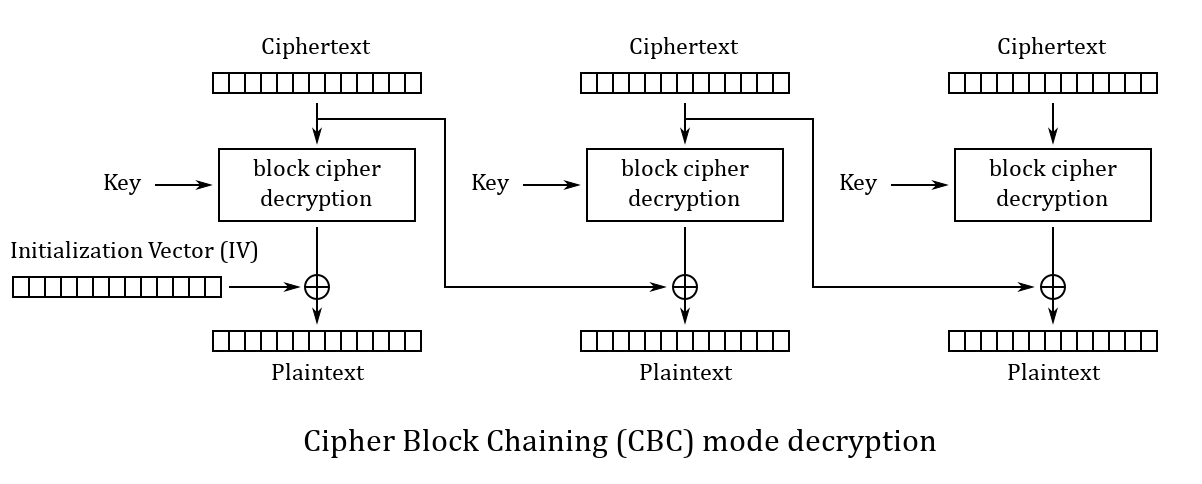
\includegraphics[width=.9\linewidth]{./img/cbc_decryption.png}
\caption{Source: Wikipedia}
\end{figure}
\end{frame}

\begin{frame}[fragile,label={sec:org55fb40f}]{CBC bitflipping attacks}
 \begin{minted}[]{ruby}
KEY = random_bytes(16)
IV = random_bytes(16)
PLAINTEXT = 'comment=1234567890&uid=3'
CIPHERTEXT = aes_cbc_encrypt(PLAINTEXT.bytes, KEY, IV)

def check(ciphertext)
  plaintext = str(aes_cbc_decrypt(ciphertext, KEY, IV))
  params = decode_query_string(plaintext)
  uid = params['uid']
  puts "checking #{plaintext.inspect}..."
  raise 'invalid string' unless uid
  uid.to_i
end
\end{minted}
\end{frame}

\begin{frame}[fragile,label={sec:org0980ee0}]{CBC bitflipping attacks}
 \begin{minted}[]{ruby}
tampered_byte = '3'.ord ^ '0'.ord
tampered = CIPHERTEXT.clone
tampered[7] ^= tampered_byte

puts "regular UID: #{check(CIPHERTEXT)}"
puts "tampered UID: #{check(tampered)}"
\end{minted}
\end{frame}

\begin{frame}[label={sec:orgb652c3a}]{CBC bitflipping attacks}
\begin{itemize}
\item Other cipher modes have similar behavior (with CTR the same block is
affected, no corruption of other blocks)
\item Solution: Sign your cookies, verify the signature to ensure it
hasn't been tampered with
\item Weak solution: Introduce a checksum to validate the integrity
\item Alternative: Use cipher mode with integrated authentication (like
AES-GCM)
\end{itemize}
\end{frame}

\begin{frame}[fragile,label={sec:orgf4ae2c1}]{Break “random access read/write” AES CTR}
 \begin{itemize}
\item AES again, but this time with a stream cipher
\item Suppose an attacker retrieves a message encrypted with AES-CTR
\item The message originates from a web application that allows editing
them and re-encrypts the result
\item This re-encryption can be done efficiently thanks to CTR allowing
you to “seek” into the keystream and allows you to patch in the
changed portion of the text
\item Luckily the attacker has access to the following API call which
returns the new ciphertext after editing:
\texttt{/edit?ciphertext=...\&offset=...\&newtext=...}
\end{itemize}
\end{frame}

\begin{frame}[fragile,label={sec:org75e32fd}]{Break “random access read/write” AES CTR}
 \begin{minted}[]{ruby}
KEY = random_bytes(16)
NONCE = random_bytes(16)
CIPHERTEXT = aes_ctr_encrypt(PLAINTEXT, KEY, NONCE)

def edit_internal(ciphertext, key, nonce, offset, newtext)
  decrypted = aes_ctr_decrypt(ciphertext, key, nonce)
  newtext.each_with_index { |byte, i| decrypted[offset + i] = byte }
  aes_ctr_encrypt(decrypted, key, nonce)
end

def edit(ciphertext, offset, newtext)
  edit_internal(ciphertext, KEY, NONCE, offset, newtext)
end
\end{minted}
\end{frame}

\begin{frame}[label={sec:orgae0cd73}]{Break “random access read/write” AES CTR}
\begin{figure}[htbp]
\centering
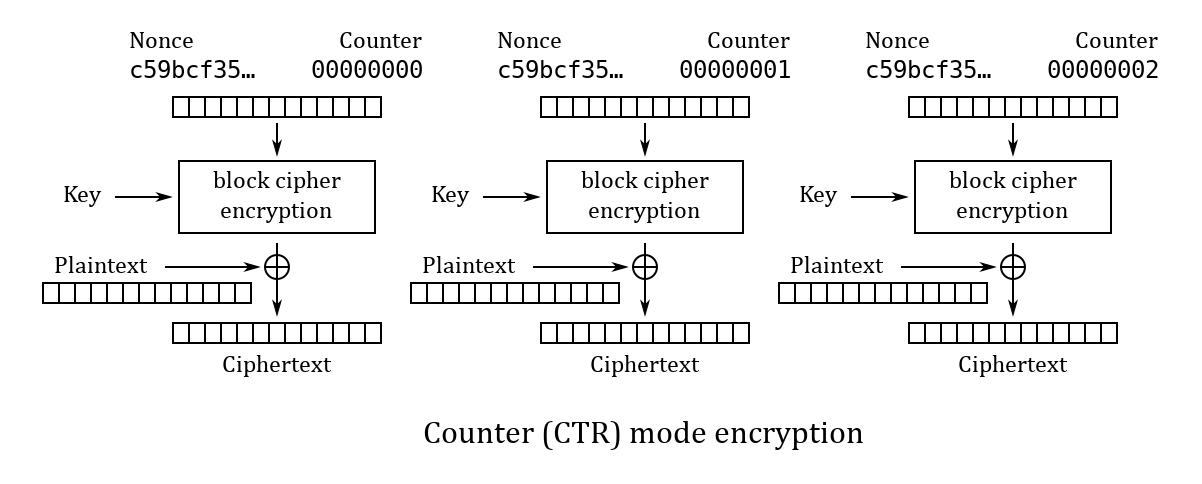
\includegraphics[width=.9\linewidth]{./img/ctr_encryption.png}
\caption{Source: Wikipedia}
\end{figure}
\end{frame}

\begin{frame}[label={sec:org972d629}]{Break “random access read/write” AES CTR}
\begin{itemize}
\item The transformation is far simpler than CBC
\item Unknown plaintext is XORed with an encrypted key stream depending on
a nonce
\item \(P_u \oplus E(k, K, N)\)
\item If the attacker XORs a known ciphertext with the existing one,
something interesting happens:
\item \(P_u \oplus E(k, K, N) \oplus P_k \oplus E(k, K, N) = P_u \oplus P_k\)
\item The attacker knows his own plaintext, but not the other one
\item \(P_u \oplus P_k \oplus P_k = P_u\)
\end{itemize}
\end{frame}

\begin{frame}[fragile,label={sec:orge1e2624}]{Break “random access read/write” AES CTR}
 \begin{minted}[]{ruby}
random_message = random_bytes(ciphertext.length)
edited_message = edit(ciphertext, 0, random_message)
puts str(xor_buffers(xor_buffers(ciphertext, edited_message),
                     random_message))
\end{minted}
\end{frame}

\begin{frame}[fragile,label={sec:org3675e85}]{Break “random access read/write” AES CTR}
 \begin{itemize}
\item Bonus: \texttt{/edit} allows a crypto-agnostic (slow) way to
decrypt the message one byte at a time
\item Suppose the attacker compares an edited ciphertext with the
original, it will always be different
\item However if the edit didn't change the content, both ciphertexts will
be the same
\item This can be used to guess part of the plaintext
\item For a byte at a given offset, guess all possible values, one of them
will reveal the plaintext byte
\item Repeat for all possible offsets and join all found plaintext bytes
\end{itemize}
\end{frame}

\begin{frame}[fragile,label={sec:org83d14b3}]{Break “random access read/write” AES CTR}
 \begin{minted}[]{ruby}
def guess_byte(ciphertext, offset)
  (0..127).each do |byte|
    return byte if ciphertext == edit(ciphertext, offset, [byte])
  end
  raise "couldn't guess byte"
end

ciphertext.size.times { |i| print guess_byte(ciphertext, i).chr }
\end{minted}
\end{frame}

\begin{frame}[label={sec:org0592f3d}]{Break “random access read/write” AES CTR}
\begin{itemize}
\item Ultimately, this attack is enabled by nonce reuse, randomize the
nonce and the keystreams no longer match up
\item For the bonus one, it should be impossible to tell if a guess was
successful or better, the resulting encryption result shouldn't be
leaked
\item Imagine if someone used this CTR property for something like FDE\ldots{}
\end{itemize}
\end{frame}

\begin{frame}[label={sec:orgeb4f0e1}]{Compression Ratio Side-Channel Attacks}
\begin{itemize}
\item This one is a side-channel attack and circumvents crypto
\item Suppose the attacker is MITM and intercepts encrypted traffic
resembling HTTP
\item Additionally to that they can inject their own content (like, by
changing the query to contain a search term)
\item They know there's a cookie inside the header and want to guess it
\item If the response is compressed before encryption, this can be done by
checking the compressed size
\end{itemize}
\end{frame}

\begin{frame}[fragile,label={sec:org6368165}]{Compression Ratio Side-Channel Attacks}
 \begin{itemize}
\item Compression generally works by finding repeating subsequences and
replacing these with something shorter
\item Suppose we compress a string containing \texttt{sessionid=abcdef}, a
subsequent \texttt{sessionid=a} will result in better compression than a
subsequent \texttt{sessionid=b}
\item Generally, the difference in reduction is measured in bits, but will
often be enough to differ by a byte
\item Oracle: Mechanism revealing a piece of information to the attacker
\end{itemize}
\end{frame}

\begin{frame}[fragile,label={sec:org94f0a1a}]{Compression Ratio Side-Channel Attacks}
 \begin{minted}[]{ruby}
def format_request(input)
  "POST / HTTP/1.1
Host: example.com
Cookie: sessionid=#{SESSIONID}
Content-Length: #{input.length}
#{input}
"
end

def oracle(input)
  key = random_bytes(16)
  nonce = random_bytes(16)
  payload = compress(format_request(input))
  aes_ctr_encrypt(payload.bytes, key, nonce).size
end
\end{minted}
\end{frame}

\begin{frame}[fragile,label={sec:org4385c75}]{Compression Ratio Side-Channel Attacks}
 \begin{minted}[]{text}
POST / HTTP/1.1
Host: example.com
Cookie: @\textcolor{red}{sessionid=}@447520626973742042756464686973742e
Content-Length: 21
@\textcolor{red}{sessionid=}@31415926
\end{minted}

\begin{minted}[]{ruby}
oracle('sessionid=31415926') #=> 117
\end{minted}
\end{frame}

\begin{frame}[fragile,label={sec:orgc1d28e4}]{Compression Ratio Side-Channel Attacks}
 \begin{minted}[]{text}
POST / HTTP/1.1
Host: example.com
Cookie: @\textcolor{red}{sessionid=4}@47520626973742042756464686973742e
Content-Length: 21
@\textcolor{red}{sessionid=4}@1415926
\end{minted}

\begin{minted}[]{ruby}
oracle('sessionid=41415926') #=> 116
\end{minted}
\end{frame}

\begin{frame}[label={sec:org08ffb33}]{Compression Ratio Side-Channel Attacks}
\begin{itemize}
\item Try each byte and record the guesses
\item A guess with a shorter compression size is likely to be correct
\item Add the guessed byte to the list of known bytes
\item If there's no good guess, either we've failed early or there's no
more bytes to guess and we're done
\item To avoid false positives, add uncompressable (random) junk
\end{itemize}
\end{frame}

\begin{frame}[fragile,label={sec:orga816509}]{Compression Ratio Side-Channel Attacks}
 \begin{minted}[]{ruby}
CHARSET = '0123456789abcdef'

def ctr_guess_byte(known)
  guesses = {}
  suffix = random_bytes(10, (128..255))
  CHARSET.each_byte do |byte|
    input = "sessionid=#{str(known + [byte] + suffix)}"
    guesses[byte] = oracle(input)
  end
  guesses.minmax_by { |_, v| v }
end
\end{minted}
\end{frame}

\begin{frame}[fragile,label={sec:orgc72352b}]{Compression Ratio Side-Channel Attacks}
 \begin{minted}[]{ruby}
known = []
loop do
  min, max = ctr_guess_byte(known)
  if min[1] == max[1]
    if known.length >= 32
      return known
    else
      known = []
      redo
    end
  end
  known << min[0]
  report_progress(str(known))
end
\end{minted}
\end{frame}

\begin{frame}[label={sec:org053f401}]{Compression Ratio Side-Channel Attacks}
\begin{itemize}
\item This is a simplified version of actual attacks, like CRIME, BREACH,
HEIST
\item No real fix for this one (other than disabling compression)
\item Note: Compressing after encryption doesn't make much sense
\item Other workarounds:
\begin{itemize}
\item Use crypto that pads to block sizes (like AES-CBC, easy to work
around)
\item Have the web server add random junk to the end (can be probably
worked around with repeated guessing)
\item Add padding that makes the length uniform (as suggested by an
expired TLS RFC draft)
\item Use XSRF tokens to mitigate the results of cookie stealing
(good luck applying that to every web application\ldots{})
\end{itemize}
\end{itemize}
\end{frame}

\section{Outro}
\label{sec:orgc8d47f1}

\begin{frame}[label={sec:orgd743485}]{Summary}
\begin{itemize}
\item There's lots of crypto out there not involving hard math
\item Good amount of well-understood attacks
\item Side-channel attacks are scary and circumvent crypto
\item Crypto systems aren't necessarily as safe as the primitives they
consist of
\item "Don't roll your own crypto" applies to primitives \alert{and}
cryptosystems
\item You should totally do the cryptopals challenges, especially if
you're a web developer
\item Crypto can be fun!
\end{itemize}
\end{frame}

\begin{frame}[label={sec:org339c960}]{Questions?}
\end{frame}
\end{document}